\fancyhead{}
\fancyfoot{}
\cfoot{\thepage}

\lhead{Anexo B.}
\chapter{Anexo B.}

% --- Fragmento: Importaciones y rutas base (train_faces) ---
\subsubsection*{Inicialización del módulo de entrenamiento}
Se presenta el bloque inicial del script \texttt{train\_faces}, donde se importan las librerías principales (\texttt{OpenCV}, \texttt{NumPy}, \texttt{DeepFace}) y los \textit{helpers} propios para detección y métricas. Además, se definen las rutas base del pipeline (\texttt{raw\_faces}, \texttt{known\_faces}, \texttt{embeddings}) y la ubicación del índice \texttt{centroids.json}. Este fragmento establece las dependencias y la estructura de directorios necesaria para el recorte de rostros y la generación de \textit{embeddings}, garantizando consistencia en el flujo de entrenamiento.

\begin{figure}[H]
    \centering
    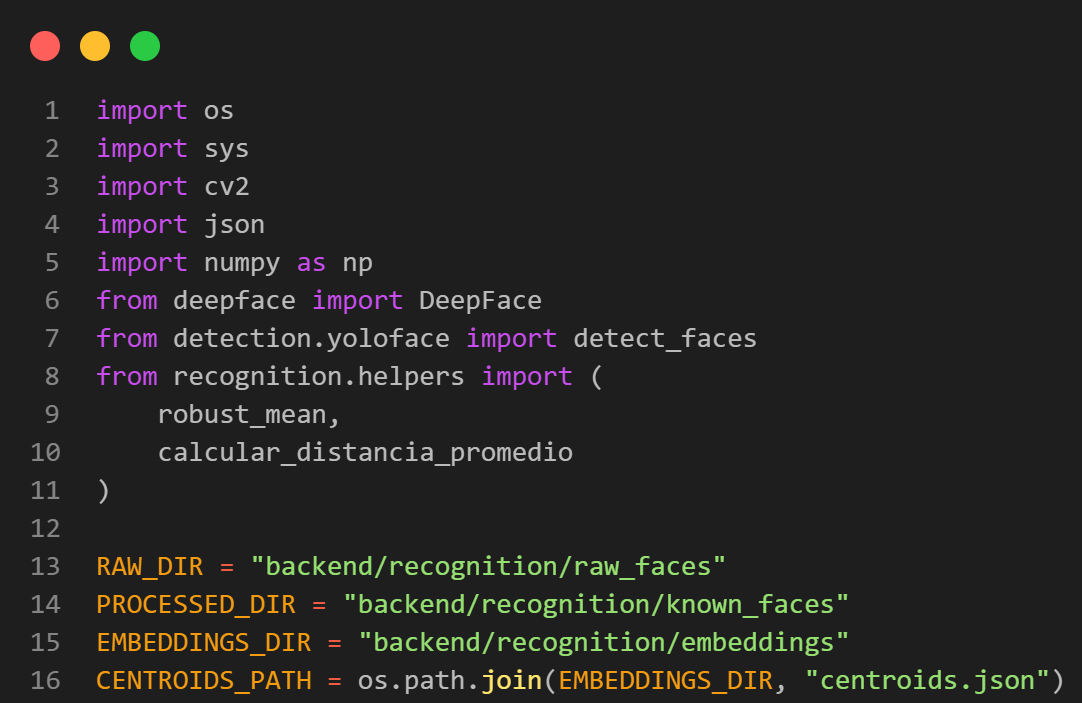
\includegraphics[width=1\textwidth]{anexos/anexo_b_img/train1.png}
    \caption{Importaciones principales y definición de rutas base del módulo de entrenamiento \texttt{train\_faces}. Se cargan dependencias para detección y representación facial y se establecen las carpetas de trabajo del pipeline [Figura propia].}
    \label{fig:train_faces_imports}
\end{figure}


% --- Fragmento: Recorte facial con YOLOv8 (train_faces) ---
\subsubsection*{Recorte y normalización de rostros}
Se muestra la función \texttt{recortar\_y\_guardar}, encargada de automatizar el preprocesamiento de imágenes por usuario (CI). El procedimiento verifica la carpeta de origen, crea el directorio de salida, recorre las imágenes válidas y, para cada archivo, aplica detección facial con YOLOv8, recorta el rostro y lo normaliza a 160\,$\times$\,160 píxeles antes de guardarlo. Este paso estandariza las entradas para el entrenamiento de embeddings.

\begin{figure}[H]
  \centering
  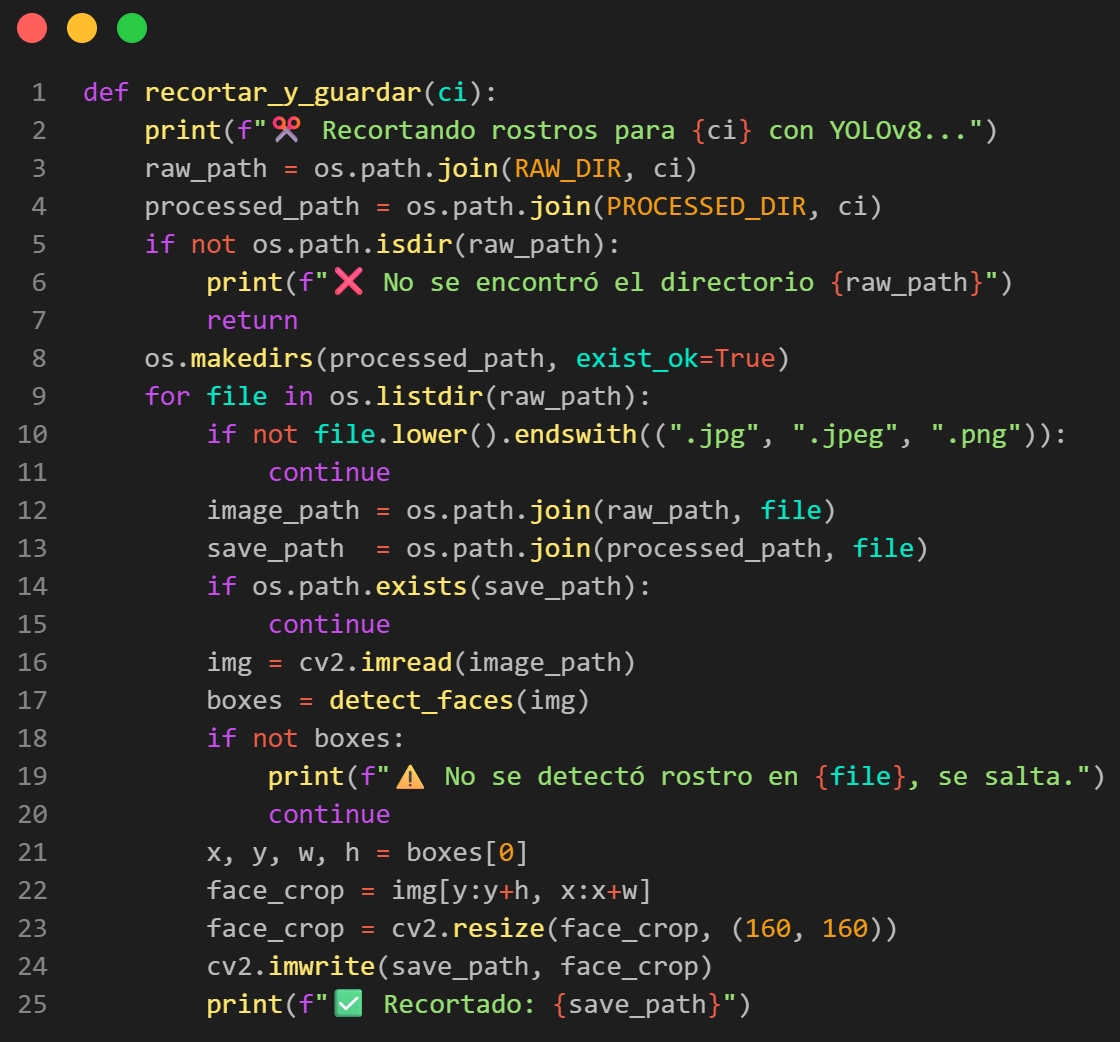
\includegraphics[width=.9\textwidth]{anexos/anexo_b_img/train2.png}
  \caption{Función \texttt{recortar\_y\_guardar} del módulo \texttt{train\_faces}, detecta rostros con YOLOv8, recorta y guarda una versión normalizada (\(160\times160\)) para generar embeddings [Figura propia].}
  \label{fig:train_faces_recorte}
\end{figure}



% --- Fragmento: Generación de embeddings (train_faces) ---
\subsubsection*{Generación de vectores de características (embeddings)}
Se observa la función \texttt{generar\_embeddings}, la cual transforma los rostros recortados en representaciones numéricas conocidas como \textit{embeddings}. El proceso comienza verificando la existencia de índices previos, luego recorre las imágenes procesadas y, mediante el modelo \texttt{ArcFace} de la librería \texttt{DeepFace}, genera un vector de 512 dimensiones por cada rostro. Estos vectores son fundamentales para el reconocimiento facial, pues permiten medir similitudes entre diferentes personas de manera precisa.

\begin{figure}[H]
    \centering
    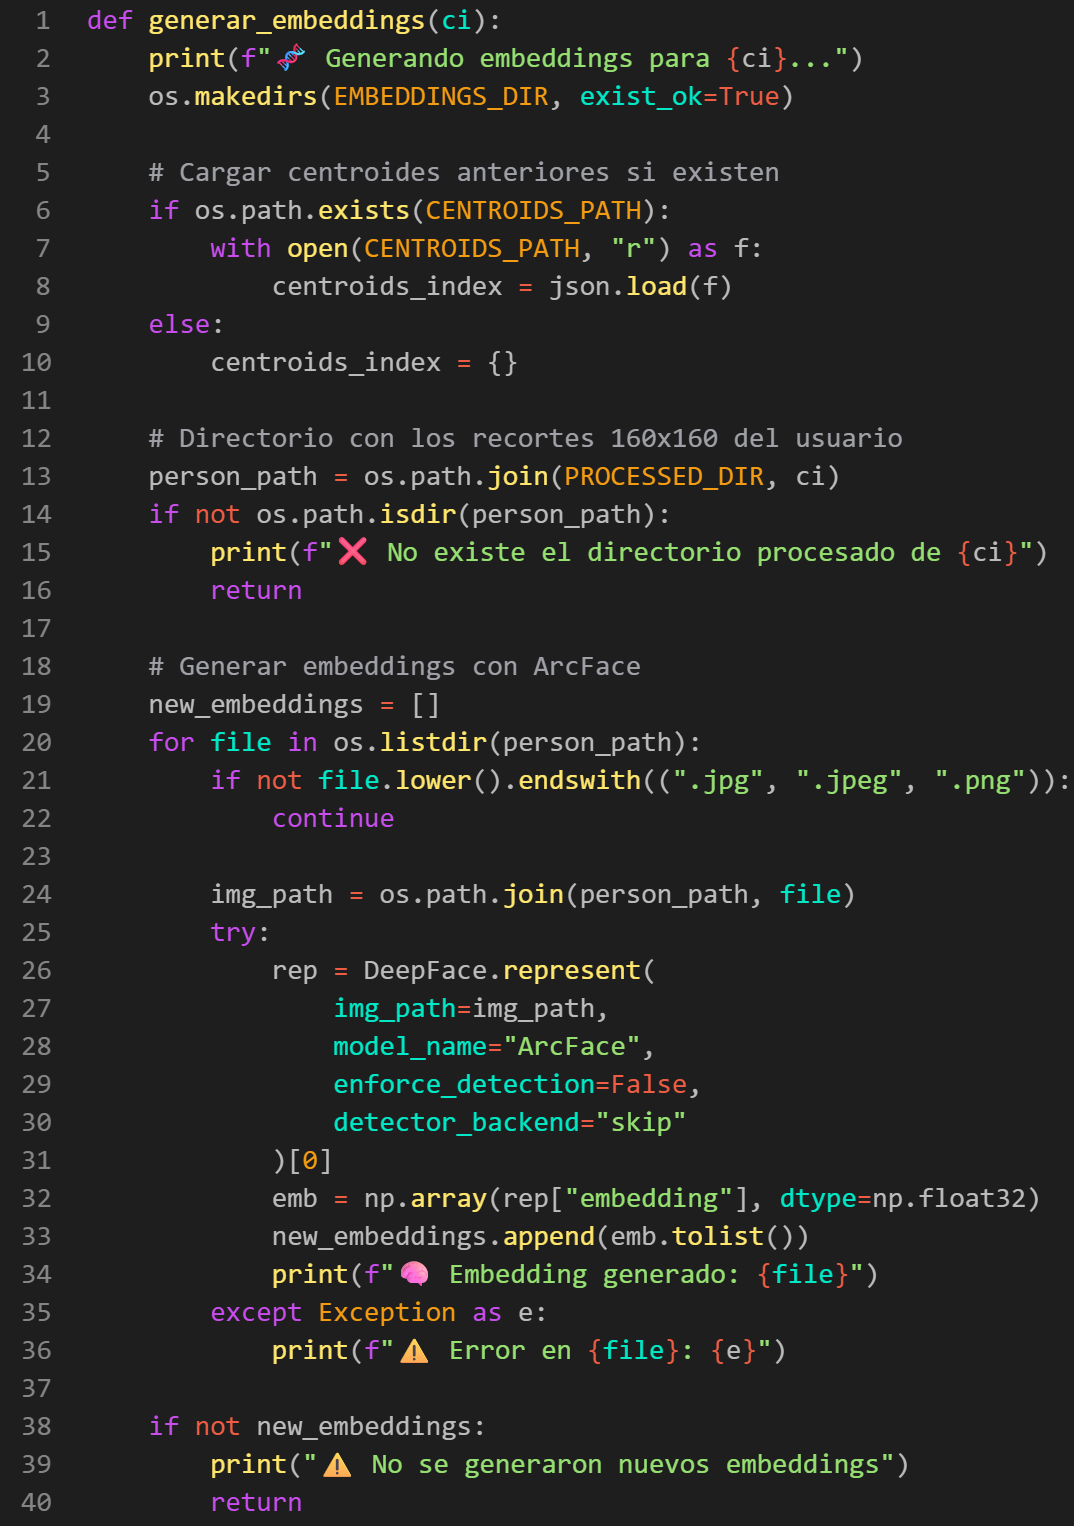
\includegraphics[width=0.9\textwidth]{anexos/anexo_b_img/train3.png}
    \caption{Fragmento del código de la función \texttt{generar\_embeddings} del módulo \texttt{train\_faces}, donde se generan las representaciones vectoriales de los rostros utilizando el modelo \texttt{ArcFace} de DeepFace [Figura propia].}
    \label{fig:train_faces_embeddings}
\end{figure}

% --- Fragmento: Cálculo de centroides y actualización del índice global (train_faces) ---
\subsubsection*{Cálculo de centroides y actualización del índice global}
En la Figura \ref{fig:train_faces_centroids} se presenta la segunda parte del procedimiento de generación de embeddings, donde se realiza el cálculo del centroide facial y se actualiza el archivo \texttt{centroids.json}. El centroide representa el promedio vectorial de todos los embeddings de un usuario, reflejando su representación facial más estable. Además, se calcula la distancia promedio intrausuario para medir la coherencia de sus imágenes. Finalmente, el script guarda los resultados en formato JSON, consolidando la información necesaria para el reconocimiento posterior.

\begin{figure}[H]
    \centering
    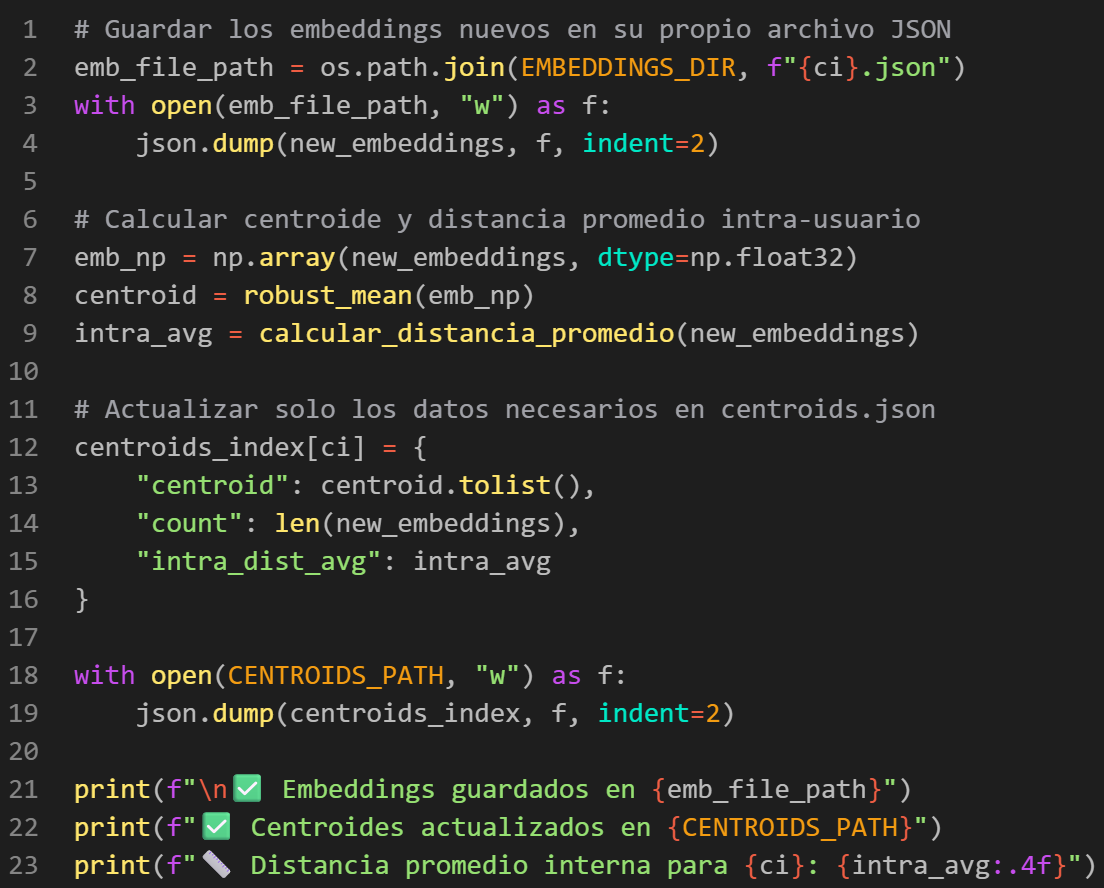
\includegraphics[width=1\textwidth]{anexos/anexo_b_img/train3.1.png}
    \caption{Fragmento del código que calcula el centroide facial y actualiza el índice global \texttt{centroids.json} con los nuevos embeddings generados [Figura propia].}
    \label{fig:train_faces_centroids}
\end{figure}

% --- Fragmento: Importaciones y configuración inicial (face_recognizer) ---
\subsubsection*{Inicialización del módulo de reconocimiento}
El fragmento mostrado a continuación contiene las importaciones esenciales y la configuración inicial del script \texttt{face\_recognizer}. Se cargan las librerías necesarias para la lectura de imágenes, manejo de archivos y operaciones matemáticas, junto con los módulos de \texttt{DeepFace} y los \textit{helpers} locales que permiten la normalización de vectores y el cálculo de la distancia coseno. Además, se definen las rutas de trabajo hacia el directorio de embeddings y el archivo \texttt{centroids.json}, el cual contiene la información de referencia para el reconocimiento facial.

\begin{figure}[H]
    \centering
    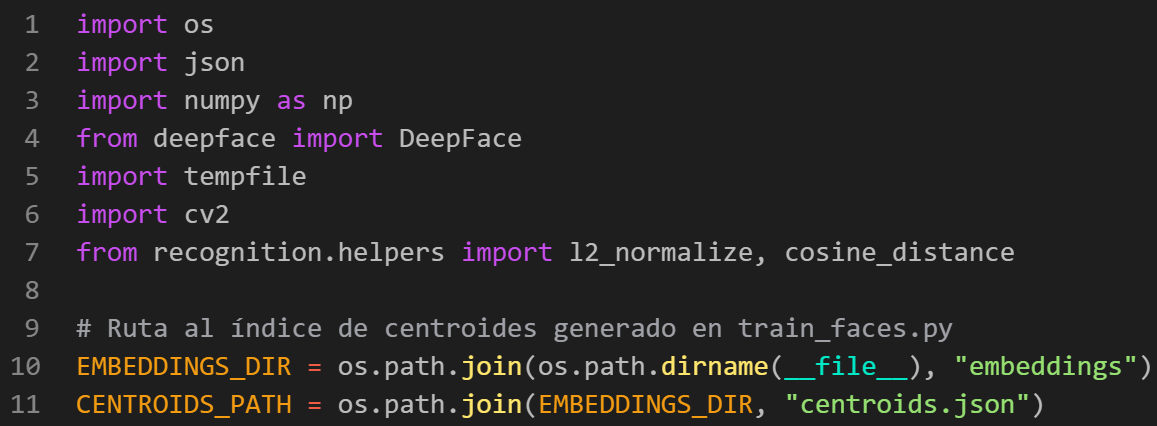
\includegraphics[width=1\textwidth]{anexos/anexo_b_img/face1.png}
    \caption{Importaciones y configuración inicial del módulo \texttt{face\_recognizer}, donde se establecen las rutas a los embeddings y centroides utilizados en la fase de reconocimiento [Figura propia].}
    \label{fig:face_recognizer_imports}
\end{figure}



% --- Fragmento: Carga y normalización de centroides (face_recognizer) ---
\subsubsection*{Carga y normalización de centroides}
El siguiente bloque corresponde a la función \texttt{load\_centroids}, que se encarga de leer el archivo \texttt{centroids.json} generado en el proceso de entrenamiento. Si el archivo no existe, el sistema emite una advertencia e indica ejecutar primero el módulo de entrenamiento. En caso contrario, carga los datos, convierte cada centroide en un arreglo NumPy y aplica una normalización L2 para uniformar las magnitudes vectoriales, asegurando coherencia en las comparaciones de similitud facial.

\begin{figure}[H]
    \centering
    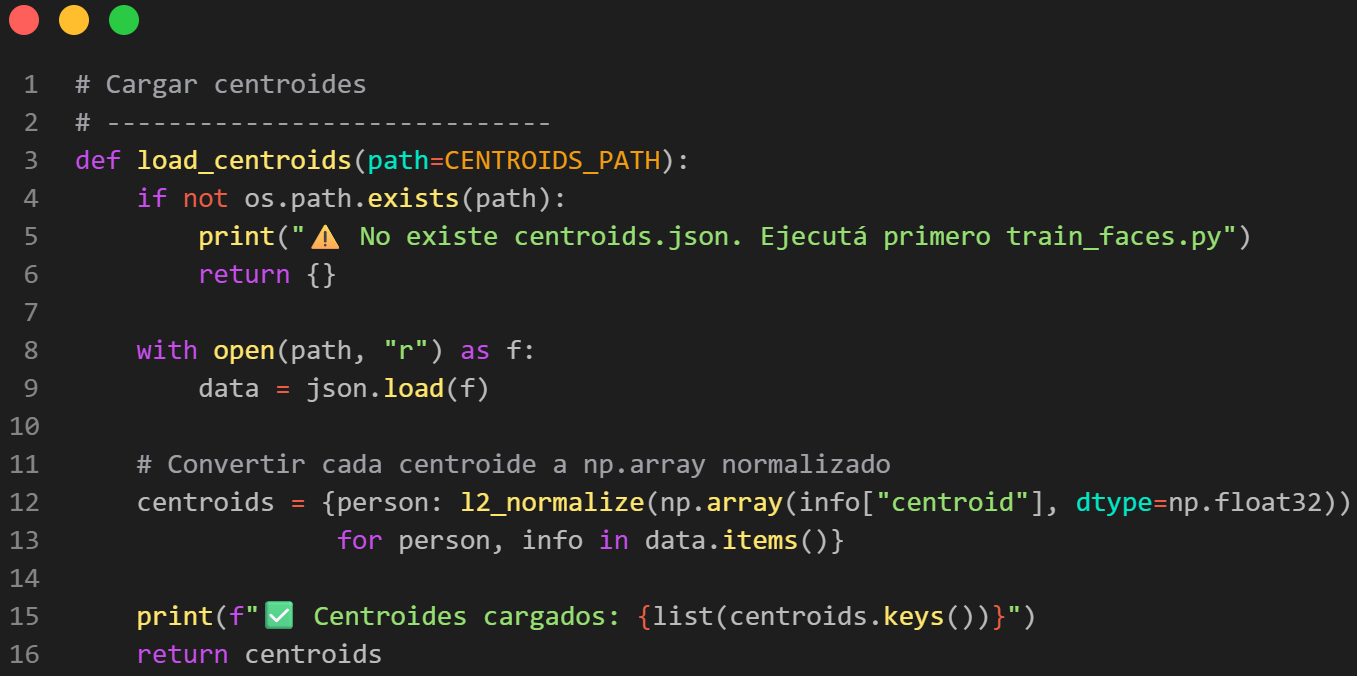
\includegraphics[width=1\textwidth]{anexos/anexo_b_img/face2.png}
    \caption{Función \texttt{load\_centroids} del módulo \texttt{face\_recognizer}, responsable de cargar y normalizar los centroides almacenados para su uso en el proceso de reconocimiento facial [Figura propia].}
    \label{fig:face_recognizer_load}
\end{figure}



% --- Fragmento: Reconocimiento individual de rostros (face_recognizer) ---
\subsubsection*{Reconocimiento individual de rostros}
Este fragmento implementa la función \texttt{recognize\_face}, responsable de identificar un rostro a partir de su recorte facial. El procedimiento crea un archivo temporal con la imagen, genera su embedding mediante el modelo \texttt{ArcFace} de \texttt{DeepFace} y normaliza el vector resultante. Posteriormente, compara el embedding con los centroides almacenados, calculando la distancia coseno para determinar el rostro más similar. Si la distancia supera un umbral definido, el sistema clasifica el rostro como desconocido. Esta función constituye el núcleo del proceso de reconocimiento facial.

\begin{figure}[H]
    \centering
    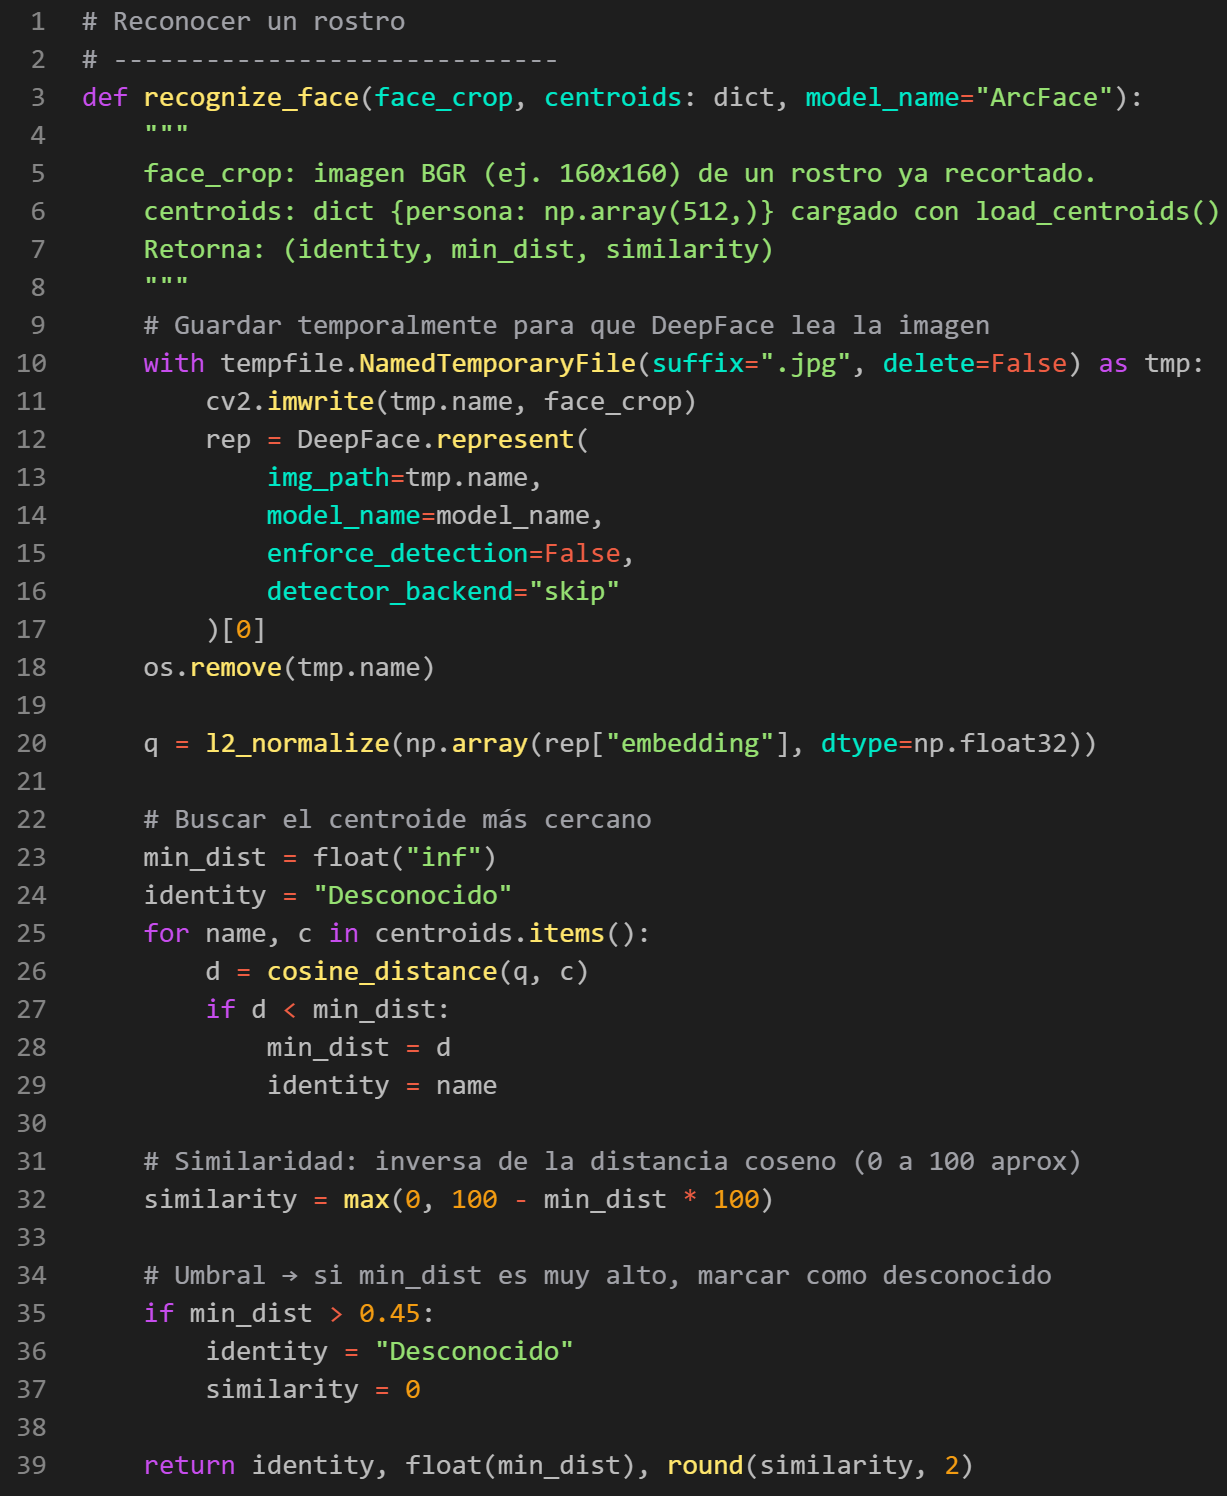
\includegraphics[width=1\textwidth]{anexos/anexo_b_img/face3.png}
    \caption{Función \texttt{recognize\_face} del módulo \texttt{face\_recognizer}, encargada de generar el embedding del rostro y compararlo con los centroides almacenados mediante la distancia coseno [Figura propia].}
    \label{fig:face_recognizer_single}
\end{figure}


% --- Fragmento: Reconocimiento múltiple de rostros (face_recognizer) ---
\subsubsection*{Reconocimiento múltiple de rostros}
La siguiente función, denominada \texttt{recognize\_faces\_from\_crops}, permite procesar simultáneamente varios rostros detectados dentro de una misma imagen. Para cada recorte facial, el método invoca la función \texttt{recognize\_face} y recopila los resultados en una lista de diccionarios que incluye el nombre identificado, la distancia mínima, el porcentaje de similitud y un valor booleano que indica si se produjo una coincidencia. Este procedimiento optimiza el rendimiento del sistema al permitir el reconocimiento de múltiples usuarios en una sola captura.

\begin{figure}[H]
    \centering
    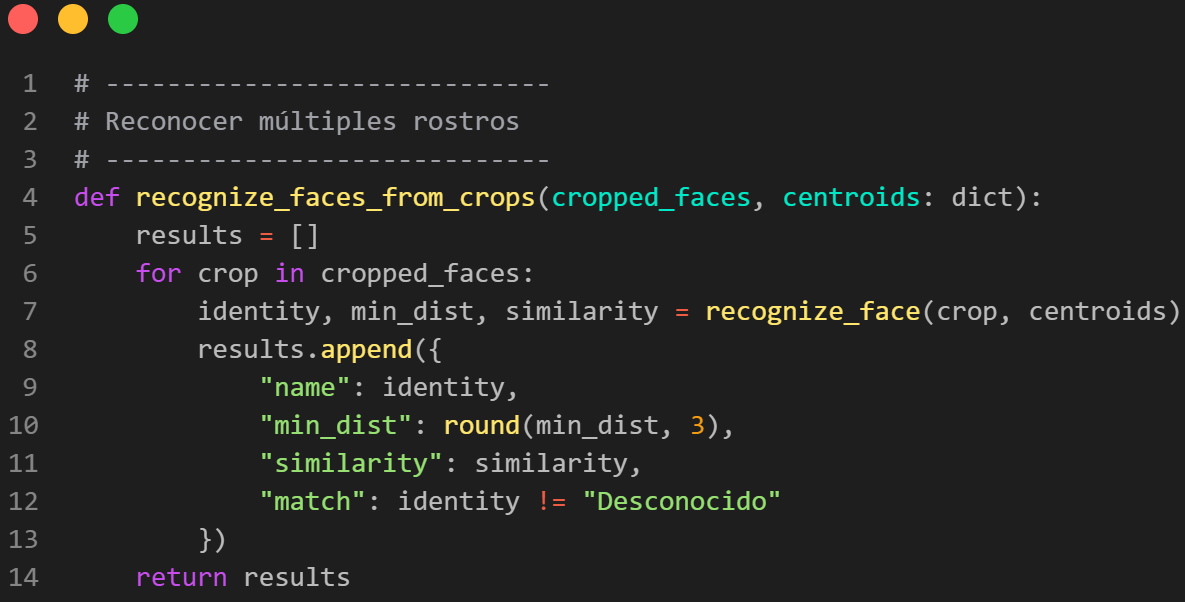
\includegraphics[width=1\textwidth]{anexos/anexo_b_img/face4.png}
    \caption{Función \texttt{recognize\_faces\_from\_crops} del módulo \texttt{face\_recognizer}, utilizada para procesar múltiples rostros detectados en una misma imagen y devolver sus resultados de identificación [Figura propia].}
    \label{fig:face_recognizer_multi}
\end{figure}
